\documentclass[letterpaper]{article}
\usepackage{flairs}%aaai
\usepackage{times}
\usepackage{helvet}
\usepackage{courier}
\usepackage{graphicx}
\usepackage{setspace}
\frenchspacing
\setlength{\pdfpagewidth}{8.5in}
\setlength{\pdfpageheight}{11in}
\pdfinfo{
/Title (Verification and Visualization of Models in Logic)
/Author (Geoff Sutcliffe, Alexander Steen, Pascal Fontaine, Jack McKeown)}
\setcounter{secnumdepth}{2}  
 \begin{document}
% This file is an adoption of the style file for AAAI Press 
% proceedings, working notes, and technical reports.  This file is made 
% with minimal changes by explicit permission from AAAI.

\title{Verification and Visualization of Models in Logic}
\author{Anon One\\
Some where\\
Some place\\
Some country\\
\And
Anon One\\
Some where\\
Some place\\
Some country\\
\And
Anon One\\
Some where\\
Some place\\
Some country\\
\And
Anon One\\
Some where\\
Some place\\
Some country}

\maketitle
\begin{abstract}
\begin{quote}
\end{quote}
\end{abstract}
%--------------------------------------------------------------------------------------------------
\section{Background}

Automated Reasoning (AR), and Automated Theorem Proving (ATP) in particular, has largely focussed
on the task of proving theorems from axioms - the derivation of conclusions that follow inevitably 
from known facts \cite{RV01-HAR}.
The axioms and conjecture to be proved (and hence become a theorem) are written in an 
appropriately expressive logic, and the proofs that are found are often similarly written in
logic \cite{SS+06}.
In this work we consider typed first-order logic in the form of \cite{Wal83,Sch85,Coh87},
%  higher-order \cite{And86}, and some 
% on-classical \cite{Pri08} logics, 
whose expressive power is sufficient for a wide range of topics \cite{Sut17}.
In the last two decades the converse task of disproving conjectures, i.e., proving that a 
conjecture is not a theorem of the axioms, has become increasingly important.
The proof is in the form of a countermodel that provides an interpretation of the formulae that 
makes the axioms {\em true} but the conjecture {\em false}.
A salient application area that harnesses this form of ATP is verification \cite{DKW08}
where countermodels are used to pinpoint the reason why a proof obligation fails, and
correspondingly point to the location of the fault in the system being verified.
Other applications include checking the consistency of an axiomatization \cite{SS+17}, and
finding a solution to a problem that is coded as a model finding problem \cite{Win82}

In addition to ATP systems that find proofs, e.g., Vampire \cite{KV13}, Leo-III \cite{SB18},
% nanoCop-M \cite{Ott21}, 
and ATP systems that find (counter)models, e.g., Paradox \cite{CS03}, FM-Darwin \cite{BF+09},
% Nipick \cite{BN10-ITP}, WHATFORNONCLASSICAL \cite{}, 
there is a need for tools that support use of the proofs and models that are output by the 
ATP systems.
This papers examines the tasks of verifying and visualizing models, and describes new tools for
these tasks.

Related work is sparse:
Model verification related work by Giles? Other? Pascal - know any from SMT?
Visualization.
No related work. Alex - know any (other than your student)?

This paper is organized as follows:
Section~\ref{TPTP} introduces the TPTP World which provides the framework and languages used
in this research.
Section~\ref{Interpretations} describes the new representation of interpretations (models being
interpretations that make certain formulae {\em true}) using the TPTP languages.
Section~\ref{Verification} provides the theory for verifying models, and describes the
implementation of that theory in a model verification tool.
Section~\ref{Visualization} introduces a novel way of visualizing interpretations, and
proposes a tool for automating the visualization of interpretations written in the TPTP language.
Section~\ref{Conclusion} concludes and discusses plans for future work.

%--------------------------------------------------------------------------------------------------
\section{The TPTP World and Language}
\label{TPTP}

The TPTP World \cite{Sut17} is a well established infrastructure that supports research, 
development, and deployment of Automated Theorem Proving (ATP) systems.
The TPTP World includes the TPTP problem library,
% \cite{Sut09}, 
the TSTP solution library,
% \cite{Sut10}, 
standards for writing ATP problems and reporting ATP solutions,
% \cite{SS+06,Sut08-KEAPPA}, 
tools and services for processing ATP problems and solutions,
% \cite{Sut10}, 
and it supports the CADE ATP System Competition (CASC).
% \cite{Sut16}.
Various parts of the TPTP World have been deployed in a range of applications,
in both academia and industry.
% Since the first release of the TPTP problem library in 1993, many researchers have used the 
% TPTP World as an appropriate and convenient basis for ATP system research and development. 
% Over the years the TPTP World has provided a platform upon which ATP users have presented their 
% needs to ATP system developers, who have then adapted their ATP systems to the users’ needs.
The web page {\tt https://www.tptp.org} provides access to all 
components.

The TPTP languages \cite{Sut22-IGPL} are one of the keys to the success of the TPTP World.
The languages are used for writing both TPTP problems and TSTP solutions, which enables convenient 
communication between different systems and researchers. 
It also enables tool exchange, tool integration, and comparable experimental results.
Originally the TPTP World supported only first-order clause normal form (CNF).
% \cite{SS98-JAR}.
Over the years full first-order form (FOF),
% \cite{Sut09}, 
typed first-order form (TFF).
% \cite{SS+12,BP13-TFF1}, 
typed extended first-order form (TXF),
% \cite{SK18}, 
typed higher-order form (THF),
% \cite{SB10,KSR16}, 
and non-classical forms (NTF),
% \footnote{%
% There are many ``non-classical logics'', including multi-valued logics \cite{Aug17},
% paraconsistent logics \cite{Pri02}, relevance logics \cite{AB75}, etc.
% In this work we are interested in those that admit Kripke interpretation \cite{Kri63},
% e.g., modal logics \cite{BBW06}.}
% \cite{SF+22} 
have been added.
% A general principle of the TPTP language is ``we provide the syntax, you provide the semantics''.
% As such, there is no a priori commitment to any semantics for the languages, although in almost 
% all cases the intended logic and semantics are well known.
All the typed languages include constructs for arithmetic.
This work applies to all the languages; TF0 (the monomorphic form of TFF) \cite{SS+12} 
% and NX0 \cite{SF+22} forms are 
is used as the examplar.

The top level building blocks of the TPTP language are {\em annotated
formulae}.
An annotated formula has the form:\\
\hspace*{0.5cm}{\em language}{\tt (}{\em name}{\tt ,}
{\em role}{\tt ,}
{\em formula}{\tt ,}
{\em source}{\tt ,}
{\em useful\_info}{\tt ).}\\
The {\em language}s supported are clause normal form ({\tt cnf}), first-order form ({\tt fof}), 
typed first-order form ({\tt tff}), and typed higher-order form ({\tt thf}).
These are used by the corresponding languages, with TXF inheriting {\tt tff} and the non-classical 
languages their corresponding underlying languages.
The {\em role}, e.g., {\tt axiom}, {\tt lemma}, {\tt conjecture},
defines the use of the formula in an ATP system.
In the {\em formula}, terms and atoms follow Prolog conventions.
%  --
% functions and predicates start with a lowercase letter or are {\tt '}single quoted{\tt '}, and 
% variables start with an uppercase letter.
The TPTP language also supports interpreted symbols, which either start with a
{\tt \$}, or are composed of non-alphanumeric characters, e.g., the truth
constants {\tt \$true} and {\tt \$false}, and integer/rational/real
numbers such as 27, 43/92, -99.66.
The basic logical connectives are
{\tt !}, {\tt ?}, {\tt \verb|~|}, {\tt |}, {\tt \&}, {\tt =>}, {\tt <=},
{\tt <=>}, and {\tt <\verb|~|>},
for
$\forall$, $\exists$, $\neg$, $\vee$, $\wedge$, $\Rightarrow$, $\Leftarrow$,
$\Leftrightarrow$, and $\oplus$ respectively.
Equality and inequality are expressed as the infix operators {\tt =} and
{\tt !=}.
The {\em source} and {\em useful\_info} are optional.
Examples problems using TF0 annotated formulae can be seen in 
Figures~\ref{TF0FiniteProblem},~\ref{TF0InfiniteProblem}, and~\ref{TF0InfiniteVerification}.
% An example annotated first-order formula, supplied from a file, is:
% \[
% \begin{minipage}{\textwidth}
% \begin{verbatim}
%     fof(union,axiom,
%         ( ! [X,A,B] :
%             ( member(X,union(A,B))
%           <=> ( member(X,A)
%               | member(X,B) ) )
%         file('SET006+0.ax',union),
%         [description('Defn of union')]).
% \end{verbatim}
% \end{minipage}
% \]
% In typical mathematical logic notation the formula is \\
% \hspace*{0.5cm}$\forall X\;\forall A\;\forall B\;(\;(X \in A\;\cup\;B) \Leftrightarrow (X \in A\;\wedge\;X \in B)\;)$

%--------------------------------------------------------------------------------------------------
\subsection{The TF0 Language}
\label{TF0}

% is a typed first-order language extended with FOOL logic constructs.
TF0 is is a typed first-order language.
Every function and predicate symbol is declared before its use, with a type signature that 
specifies the types of the symbol’s arguments and result.
The TX0 types are 
(i)~the predefined types {\tt \$i} for individuals and {\tt \$o} for booleans; 
(ii)~the predefined arithmetic types {\tt \$int}, {\tt \$rat}, and {\tt \$real}; 
(iii)~user-defined types that have been declared to be of the kind {\tt \$tType}.
TF0 type signatures are 
(i)~individual types;
(ii)~function types from non-boolean argument types to result types;
(iii)~predicate types from non-boolean argument types to boolean.
The equality predicates {\tt =} and {\tt !=} are ad hoc polymorphic over all types, and the types 
of arithmetic predicates and functions are ad hoc polymorphic over the arithmetic types.
% TX0 formulae are those of first-order logic, extended to allow boolean variables and terms.
% TX0 additionally supports tuples, conditional expressions, and let expressions, but they are
% not used in this paper (see \cite{SK18} for the details).
Figure~\ref{TF0FiniteProblem} is a problem in TF0 (which has a finite countermodel - see 
Section~\ref{Interpretations}), and Figure~\ref{TF0InfiniteProblem} is another problem 
in TF0 (which has an model with an infinite domain - see Section~\ref{Interpretations}).
% not using any of the extended language features
% (those feature will come into play later).

\begin{figure}[htbp]
\scriptsize
\setstretch{0.8}
\begin{verbatim}
%-------------------------------------------------------
tff(man_type,type,           man: $tType ).
tff(grade_type,type,         grade: $tType ).
tff(john_decl,type,          john: man ).
tff(a_decl,type,             a: grade ).
tff(f_decl,type,             f: grade ).
tff(grade_of_decl,type,      grade_of: man > grade ).
tff(created_equal_decl,type, 
    created_equal: ( man * man ) > $o ).

tff(all_created_equal,axiom,
    ! [H1: man,H2: man] : created_equal(H1,H2) ).

tff(john_failed,axiom,
    grade_of(john) = f ).

tff(someone_got_an_a,axiom,
    ? [H: man] : grade_of(H) = a ).

tff(distinct_grades,axiom,
    a != f ).

tff(equality_lost,conjecture,
    ! [H1: man,H2: man] :
      ( created_equal(H1,H2)
    <=> ( H1 = H2 ) ) ).
%-------------------------------------------------------
\end{verbatim}
\caption{A TF0 problem (with a finite countermodel)}
\label{TF0FiniteProblem}
\end{figure}

\begin{figure}[htbp]
\scriptsize
\setstretch{0.8}
\begin{verbatim}
%-------------------------------------------------------
tff(person_type,type,        person: $tType ).
tff(bob_decl,type,           bob: person ).
tff(child_of_decl,type,      child_of: person > person ).
tff(is_descendant_decl,type, 
    is_descendant: ( person * person ) > $o ).

tff(descendents_different,axiom,
    ! [A: person,D: person] : 
      ( is_descendant(A,D) => A != D ) ).

tff(descendent_transitive,axiom,
    ! [A: person,C: person,G: person] :
      ( ( is_descendant(A,C) & is_descendant(C,G) ) 
     => is_descendant(A,G) ) ).

tff(child_is_descendant,axiom,
    ! [P: person] : is_descendant(P,child_of(P)) ).

tff(all_have_child,axiom,
    ! [P: person] : ? [C: person] : C = child_of(P) ).
%-------------------------------------------------------
\end{verbatim}
\caption{A TF0 problem (with an infinite model)}
\label{TF0InfiniteProblem}
\end{figure}

%--------------------------------------------------------------------------------------------------
% \subsection{The NXF Language}
% \label{NXF}

%--------------------------------------------------------------------------------------------------
\section{Representing Interpretations}
\label{Interpretations}

An interpretation of a formulae in a classical logic consists of domains (one for each type -
just one domain in the case of untyped logic), and interpretation of the symbols of the 
formulae wrt the domains \cite{Hun96}.
The domains may be finite or infinite.
% A Kripke interpretation of a formulae in a non-classical logic consists of a set or worlds,
% an accessibility relation between those worlds, and a classical logic interpretation within each
% world \cite{}.
% The set of worlds may be finite or infinite.
In earlier work \cite{SS+06} a TPTP format for interpretations with finite domains was defined,
and has been adopted by some ATP systems that find finite models, e.g., Paradox and Vampire.
More recently the need for a format for classical logic interpretations with infinite domains,
and for a format for Kripke interpretations \cite{Kri63} of formulae written in the NTF language, 
has led to the development of a new format for interpretations using the TPTP languages.

Figure~\ref{TF0FiniteInterpretation} is an interpretation with a finite domain - it is a 
countermodel for the problem in Figure~\ref{TF0FiniteProblem}.

\begin{figure}[htbp]
\scriptsize
\setstretch{0.8}
\begin{verbatim}
%-------------------------------------------------------
tff(man_type,type,           man: $tType ).
tff(grade_type,type,         grade: $tType ).
tff(john_decl,type,          john: man ).
tff(a_decl,type,             a: grade ).
tff(f_decl,type,             f: grade ).
tff(grade_of_decl,type,      grade_of: man > grade ).
tff(created_equal_decl,type, 
    created_equal: ( man * man ) > $o ).

tff(d2man_type,type,         d2man: $tType).
tff(d_grade_type,type,       d_grade: $tType).
tff(d2man_decl,type,      d2man: d2man > man ).
tff(d_grade_decl,type,    
    d_grade: d_grade > grade ).

tff(d_john_decl,type,        d_john: d2man ).
tff(d_gotA_decl,type,       d_gotA: d2man ).
tff(d_a_decl,type,           d_a: d_grade ).
tff(d_f_decl,type,           d_f: d_grade ).

tff(equality_lost,interpretation,
%----Man domain elements are d_john and d_gotA
    ( ( ! [X: d2man] : ( X = d_john | X = d_gotA )
      & $distinct(d_john,d_gotA)
%----The type promoter is a bijection 
      & ! [X: d2man,Y: d2man] : 
          ( d2man(X) = d2man(Y) => X = Y )
      & ! [X: man] : ? [DX: d2man] : d2man(DX) = X
%----Grade domain elements are d_a and d_f
      & ! [X: d_grade]: ( X = d_a | X = d_f )
      & $distinct(d_a,d_f)
%----The type promoter is a bijection 
      & ! [X: d_grade,Y: d_grade] : 
          ( d_grade(X) = d_grade(Y) => X = Y )
      & ! [X: grade] : 
        ? [DX: d_grade] : d_grade(DX) = X )
%----Interpret terms via the type-promoted domain
    & ( a = d_grade(d_a)
      & f = d_grade(d_f)
      & john = d2man(d_john)
      & grade_of(d2man(d_john)) = d_grade(d_f)
      & grade_of(d2man(d_gotA)) = d_grade(d_a) )
%----Interpret atoms as true of false
    & ( created_equal(d2man(d_john),d2man(d_john))
      & created_equal(d2man(d_john),d2man(d_gotA))
      & created_equal(d2man(d_gotA),d2man(d_john))
      & created_equal(d2man(d_gotA),d2man(d_gotA)) ) 
    ) ).
%----If John was not equal to the man who got an A:
%----& ~ created_equal(d2man(d_john),d2man(d_gotA))
%----& ~ created_equal(d2man(d_gotA),d2man(d_john))
%-------------------------------------------------------
\end{verbatim}
\caption{A TF0 interpretation with a finite domain}
\label{TF0FiniteInterpretation}
\end{figure}

Figure~\ref{TF0InfiniteInterpretation} is an interpretation with a finite domain - it is a 
countermodel for the problem in Figure~\ref{TF0InfiniteProblem}.

\begin{figure}[htbp]
\scriptsize
\setstretch{0.8}
\begin{verbatim}
%-------------------------------------------------------
tff(person_type,type,        person: $tType ).
tff(bob_decl,type,           bob: person ).
tff(child_of_decl,type,      child_of: person > person ).
tff(is_descendant_decl,type, 
    is_descendant: ( person * person ) > $o ).

tff(int2person_decl,type, int2person: $int > person ).

tff(people,interpretation,
%----Domain for type person is the integers
    ( ! [P: person] : ? [I: $int] : int2person(I) = P
%----The type promoter is a bijection
    & ! [I1: $int,I2: $int] : 
        ( int2person(I1) = int2person(I2) 
       => I1 = I2 )
%----Mapping people to integers. 
    & bob = int2person(0)
    & ! [I: $int] : 
        child_of(int2person(I)) = int2person($sum(I,1))
%----Interpretation of descendancy
    & ! [A: $int,D: $int] : 
        ( is_descendant(int2person(A),int2person(D)) 
      <=> $less(A,D) ) ) ).
%-------------------------------------------------------
\end{verbatim}
\caption{A TF0 interpretation with an infinite domain}
\label{TF0InfiniteInterpretation}
\end{figure}

%--------------------------------------------------------------------------------------------------
% \subsection{Kripke Interpretations}
% \label{Kripke}

%--------------------------------------------------------------------------------------------------
\section{Model Verification}
\label{Verification}

Figure~\ref{TF0InfiniteVerification} is an interpretation with a finite domain - it is a
countermodel for the problem in Figure~\ref{TF0FiniteProblem}.

\begin{figure}[htbp]
\scriptsize
\setstretch{0.8}
\begin{verbatim}
%-------------------------------------------------------
tff(person_type,type,        person: $tType ).
tff(bob_decl,type,           bob: person ).
tff(child_of_decl,type,      child_of: person > person ).
tff(is_descendant_decl,type, 
    is_descendant: ( person * person ) > $o ).

tff(int2person_decl,type,   int2person: $int > person ).

tff(people,axiom,
    ( ( ! [P: person] : ? [I: $int] : int2person(I) = P
      & ! [I1: $int,I2: $int] : 
          ( int2person(I1) = int2person(I2) 
         => I1 = I2 ) )
    & bob = int2person(0)
    & ! [I: $int] : 
        child_of(int2person(I)) = int2person($sum(I,1))
    & ! [A: $int,D: $int] : 
        ( is_descendant(int2person(A),int2person(D)) 
      <=> $less(A,D) ) ) ).

tff(prove_formulae,conjecture,
    ( ! [A: person,D: person] : 
        ( is_descendant(A,D) => A != D )
    & ! [A: person,C: person,G: person] :
        ( ( is_descendant(A,C) & is_descendant(C,G) )
       => is_descendant(A,G) )
    & ! [P: person] : is_descendant(P,child_of(P))
    & ! [P: person] : ? [C: person] : C = child_of(P) 
    ) ).
%-------------------------------------------------------
\end{verbatim}
\caption{A TF0 verification problem for a countermodel with an infinite domain}
\label{TF0InfiniteVerification}
\end{figure}

%--------------------------------------------------------------------------------------------------
\section{Interpretation Visualization}
\label{Visualization}

Figure~\ref{TF0FiniteIIV} is a visualization of the countermodel shown in 
Figure~\ref{TF0FiniteInterpretation}.

\begin{figure}[htbp]
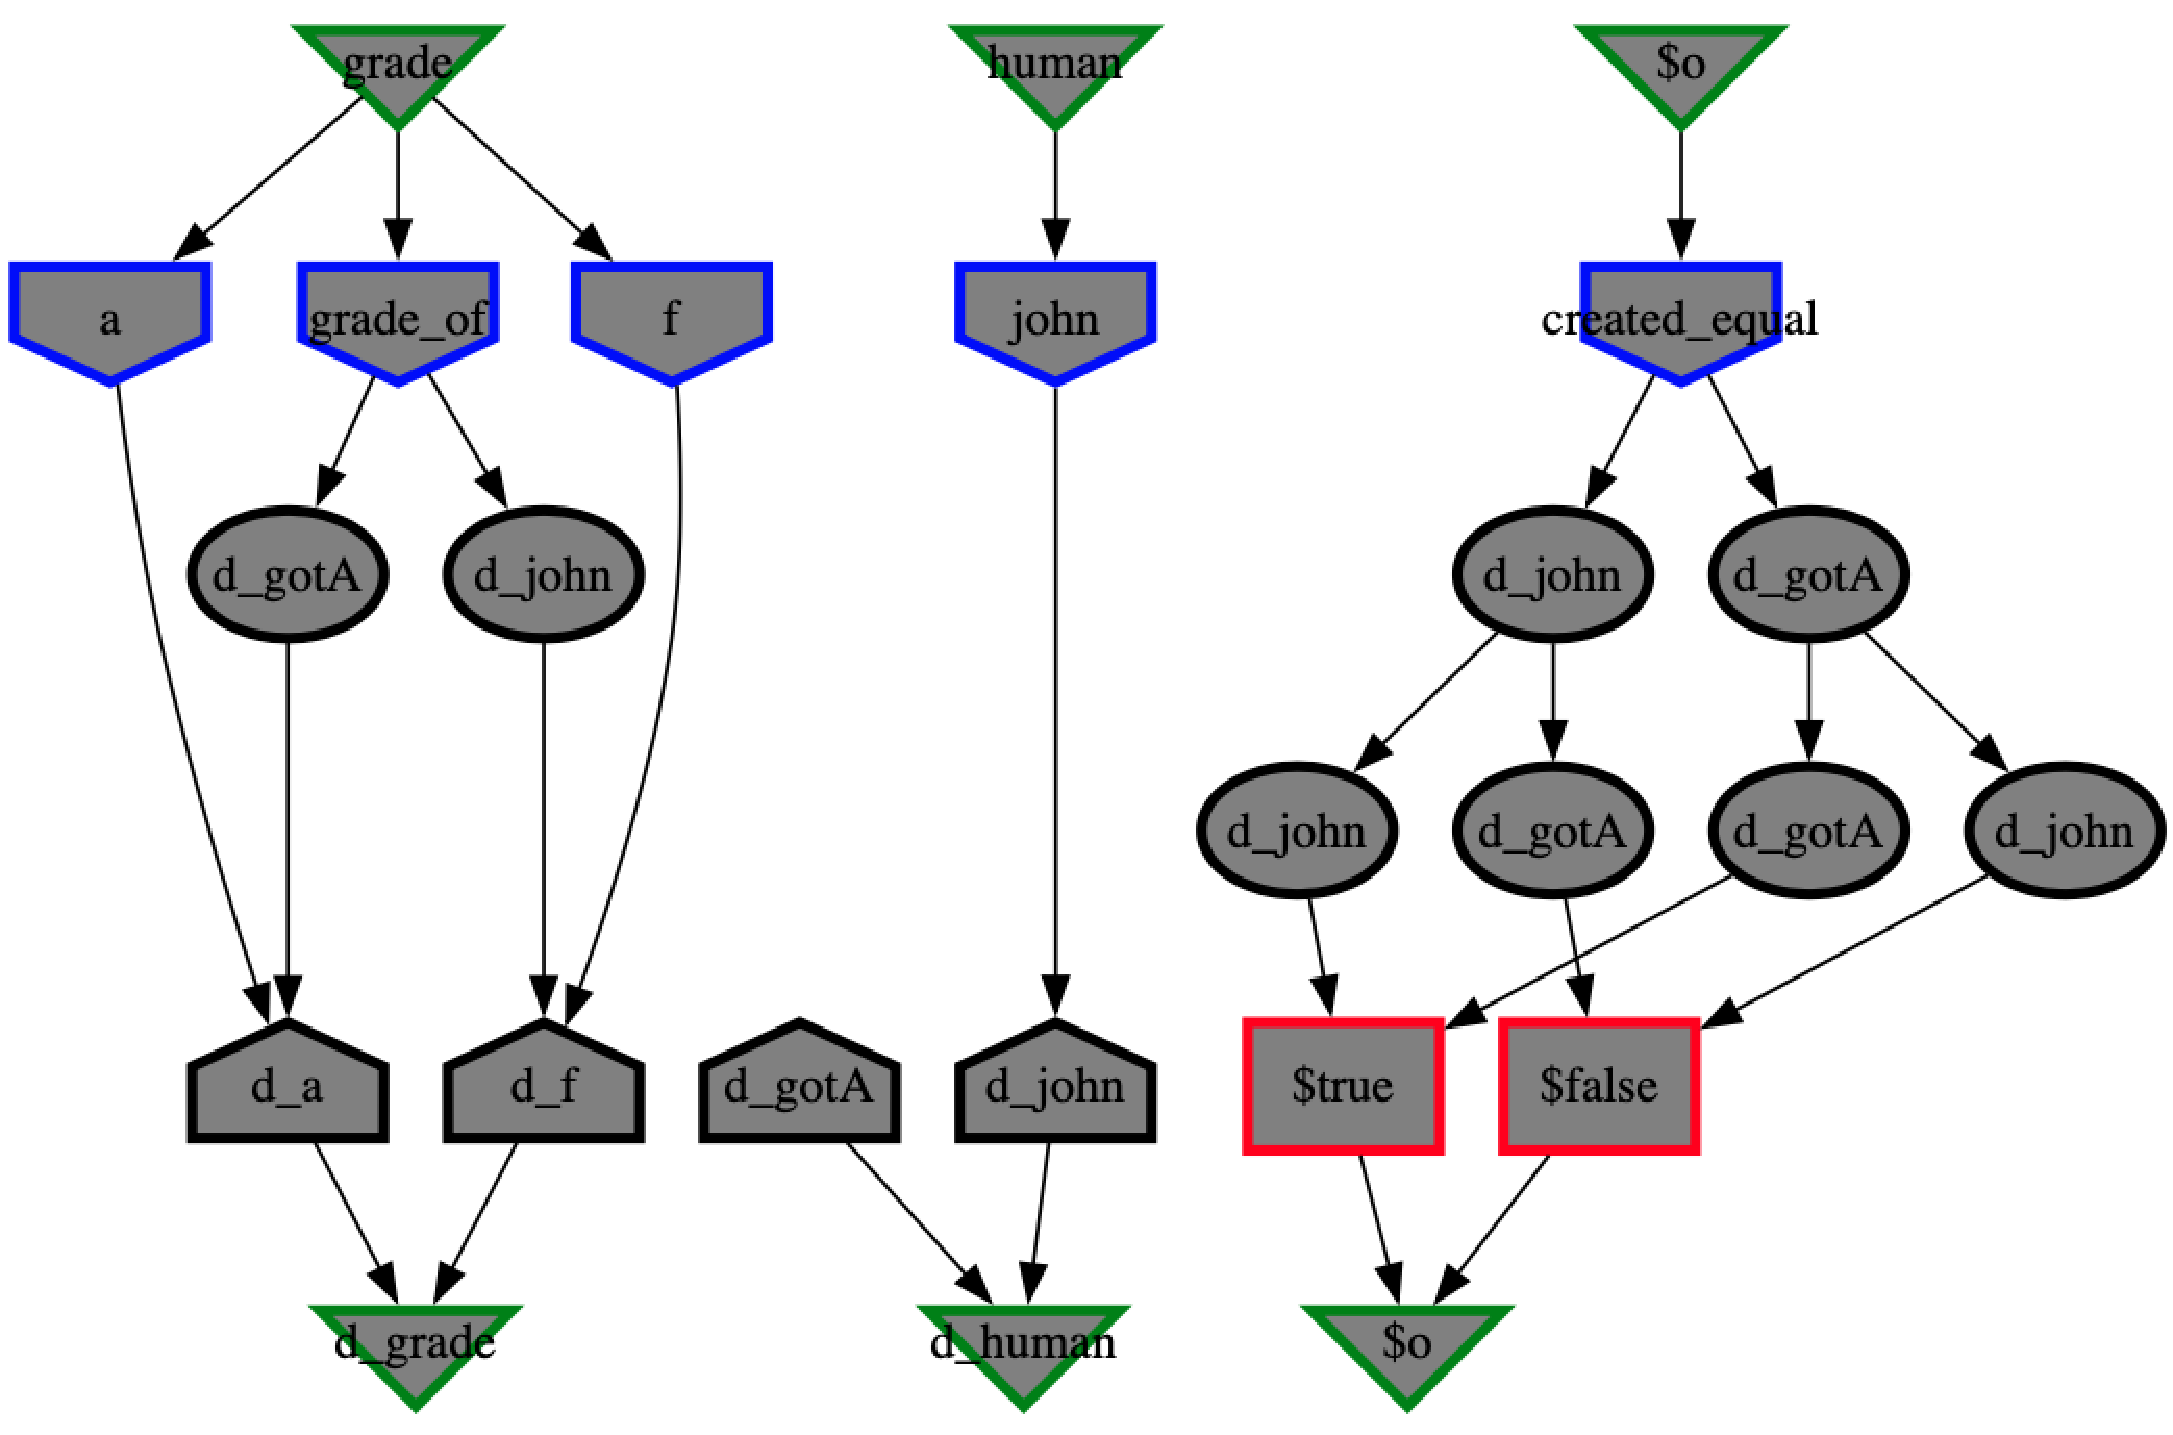
\includegraphics[width=\columnwidth]{IIV.pdf}
\caption{A visualization of an interpretation with a finite domain}
\label{TF0FiniteIIV}
\end{figure}

What about infinite domains?

%--------------------------------------------------------------------------------------------------
\section{Conclusion}
\label{Conclusion}

%--------------------------------------------------------------------------------------------------
\bibliographystyle{flairs}
\bibliography{Bibliography.bib}
%--------------------------------------------------------------------------------------------------
\end{document}
%--------------------------------------------------------------------------------------------------
%% \section{Formatting Requirements in Brief}
%% We need source and PDF files that can be used in a variety of ways and can be output on a variety of devices. FLAIRS imposes some requirements on your source and PDF files that must be followed. Most of these requirements are based on our efforts to standardize conference manuscript properties and layout. These requirements are as follows, and all papers submitted to FLAIRS for publication must comply:
%% 
%% \begin{itemize}
%% \item Your .tex file must compile in PDF\LaTeX{} --- \textbf{ no .ps or .eps figure files.}
%% \item All fonts must be embedded in the PDF file --- \textbf{ this includes your figures.}
%% \item Modifications to the style sheet (or your document) in an effort to avoid extra page  are NOT allowed.
%% \item No type 3 fonts may be used (even in illustrations).
%% \item Your title must follow US capitalization rules.
%% \item \LaTeX{} documents must use the Times or Nimbus font package (do not use Computer Modern for the text of your paper).
%% \item Fonts that require non-English language support (CID and Identity-H) must be converted to outlines or removed from the document (even if they are in a graphics file embedded in the document). 
%% \item Two-column format is required for all papers.
%% \item The paper size for final submission must be US letter. No exceptions.
%% \item The source file must exactly match the PDF.
%% \item The document margins must be as specified in the formatting instructions.
%% \item The number of pages and the file size must be as specified for your event.
%% \item No document may be password protected.
%% \item Neither the PDFs nor the source may contain any embedded links or bookmarks.
%% \item Your source and PDF must not have any page numbers, footers, or headers.
%% \item Your PDF must be compatible with Acrobat 5 or higher.
%% \item Your \LaTeX{} source file (excluding references) must consist of a \textbf{single} file (use of the ``input" command is not allowed.
%% \item Your graphics must be sized appropriately outside of \LaTeX{} (do not use the ``clip" command) .
%% \end{itemize}
%% 
%% If you do not follow the above requirements, it is likely that we will be unable to publish your paper.
%% 
%% \section{What Files to Submit}
%% You must submit the following items to ensure that your paper is published:
%% \begin{itemize}
%% \item A fully-compliant PDF file.
%% \item Your  \LaTeX{}  source file submitted as a \textbf{single} .tex file (do not use the ``input" command to include sections of your paper --- every section must be in the single source file). The only exception is the bibliography, which you may include separately. Your source must compile on our system, which includes the standard \LaTeX{} support files.
%% \item All your graphics files.
%% \item The \LaTeX{}-generated files (e.g. .aux and .bib file, etc.) for your compiled source.
%% \item All the nonstandard style files (ones not commonly found in standard \LaTeX{} installations) used in your document (including, for example, old algorithm style files). If in doubt, include it.
%% \end{itemize}
%% 
%% Your \LaTeX{} source will be reviewed and recompiled on our system (if it does not compile, you may incur late fees).   \textbf{Do not submit your source in multiple text files.} Your single \LaTeX{} source file must include all your text, your bibliography (formatted using flairs.bst), and any custom macros. Accompanying this source file, you must also supply any nonstandard (or older) referenced style files and all your referenced graphics files. 
%% 
%% Your files should work without any supporting files (other than the program itself) on any computer with a standard \LaTeX{} distribution. Place your PDF and source files in a single tar, zipped, gzipped, stuffed, or compressed archive. Name your source file with your last (family) name.
%% 
%% \textbf{Do not send files that are not actually used in the paper.} We don't want you to send us any files not needed for compiling your paper, including, for example, this instructions file, unused graphics files, and so forth.  
%% 
%% \section{Using \LaTeX{} to Format Your Paper}
%% 
%% The latest version of the FLAIRS style file is available on FLAIRS's website. Download this file and place it in a file named ``flairs.sty" in the \TeX\ search path. Placing it in the same directory as the paper should also work. You must download the latest version.
%% 
%% The following packages are incompatible with flairs.sty and/or flairs.bst and must not be used (this list is not exhaustive --- there are others as well):
%% \begin{itemize}
%% \item hyperref
%% \item natbib
%% \item geometry
%% \item titlesec
%% \item layout
%% \item caption
%% \item titlesec
%% \item T1 fontenc package (install the CM super fonts package instead)
%% \end{itemize}
%% 
%% \subsection{Illegal Commands}
%% The following commands may not be used in your paper:
%% \begin{itemize}
%% \item \textbackslash input
%% \item \textbackslash vspace (when used before or after a section or subsection)
%% \item \textbackslash addtolength 
%% \item \textbackslash columnsep
%% \item \textbackslash top margin (or text height or addsidemargin or even side margin)
%% \end{itemize}
%% 
%% \subsection{Paper Size, Margins, and Column Width}
%% Papers must be formatted to print in two-column format on 8.5 x 11 inch US letter-sized paper. The margins must be exactly as follows: 
%% \begin{itemize}
%% \item Top margin: .75 inches
%% \item Left margin: .75 inches
%% \item Right margin: .75 inches
%% \item Bottom margin: 1.25 inches
%% \end{itemize} 
%% 
%% 
%% The default paper size in most installations of \LaTeX{} is A4. However, because we require that your electronic paper be formatted in US letter size, you will need to alter the default for this paper to US letter size. Assuming you are using the 2e version of \LaTeX{}, you can do this by including the [letterpaper] option at the beginning of your file: 
%% \textbackslash documentclass[letterpaper]{article}. 
%% 
%% This command is usually sufficient to change the format. Sometimes, however, it may not work. Use PDF\LaTeX{} and include
%% \textbackslash setlength\{\textbackslash pdfpagewidth\}\{8.5in\}
%% \textbackslash setlength\{\textbackslash pdfpageheight\}\{11in\}
%% in your preamble. 
%% 
%% \textbf{Do not use the Geometry package to alter the page size.} Use of this style file alters flairs.sty and will result in your paper being rejected. 
%% 
%% 
%% \subsubsection{Column Width and Margins.}
%% To ensure maximum readability, your paper must include two columns. Each column should be 3.3 inches wide (slightly more than 3.25 inches), with a .375 inch (.952 cm) gutter of white space between the two columns. The flairs.sty file will automatically create these columns for you. 
%% 
%% \subsection{Overlength Papers}
%% If your paper is too long, turn on \textbackslash frenchspacing, which will reduce the space after periods. Next,  shrink the size of your graphics. Use \textbackslash centering instead of \textbackslash begin\{center\} in your figure environment. If these two methods don't work, you may minimally use the following. For floats (tables and figures), you may minimally reduce \textbackslash floatsep, \textbackslash textfloatsep, \textbackslash abovecaptionskip, and \textbackslash belowcaptionskip. For mathematical environments, you may minimally reduce \textbackslash abovedisplayskip, \textbackslash belowdisplayskip, and \textbackslash arraycolsep. You may also alter the size of your bibliography by inserting \textbackslash fontsize\{9.5pt\}\{10.5pt\} \textbackslash selectfont
%% right before the bibliography. 
%% 
%% Commands that alter page layout are forbidden. These include \textbackslash columnsep, \textbackslash topmargin, \textbackslash topskip, \textbackslash textheight, \textbackslash textwidth, \textbackslash oddsidemargin, and \textbackslash evensizemargin (this list is not exhaustive). If you alter page layout, you will be required to pay the page fee \textit{plus} a reformatting fee. Other commands that are questionable and may cause your paper to be rejected include  \textbackslash parindent, and \textbackslash parskip. Commands that alter the space between sections are also questionable. The title sec package is not allowed. Regardless of the above, if your paper is obviously ``squeezed" it is not going to to be accepted. Before using every trick you know to make your paper a certain length, try reducing the size of your graphics or cutting text instead.
%% 
%% \subsection{Credits}
%% Any credits to a sponsoring agency should appear in the acknowledgments section, unless the agency requires different placement. If it is necessary to include this information on the front page, use
%% \textbackslash thanks in either the \textbackslash author or \textbackslash title commands.
%% For example:
%% \begin{quote}
%% \begin{small}
%% \textbackslash title\{Very Important Results in AI\textbackslash thanks\{This work is
%%  supported by everybody.\}\}
%% \end{small}
%% \end{quote}
%% Multiple \textbackslash thanks commands can be given. Each will result in a separate footnote indication in the author or title with the corresponding text at the botton of the first column of the document. Note that the \textbackslash thanks command is fragile. You will need to use \textbackslash protect.
%% 
%% Please do not include \textbackslash pubnote commands in your document.
%% 
